%%%%%%%%%%%%%%%%%%%%%%%%%%%%%%%%%%%%%%%%%%%%%%%%%%%%%%%%%%%%%%%%%%%%%%%%%%%%%%%%
\begin{frame}{Context}
Multiagent problems
\begin{columns}
\begin{column}{0.45\textwidth}
\begin{itemize}
\item stock market
\item group of robots
\end{itemize}
\end{column}
\pause
\begin{column}{0.45\textwidth}
\begin{itemize}
\item predictive
\item prescriptive
\end{itemize}
\end{column}
\end{columns}

\bigskip\bigskip
\pause
Game-theoretic approach
\begin{itemize}
\item selfish agents
\item different solution concepts
\end{itemize}
\end{frame}
%%%%%%%%%%%%%%%%%%%%%%%%%%%%%%%%%%%%%%%%%%%%%%%%%%%%%%%%%%%%%%%%%%%%%%%%%%%%%%%%
%%%%%%%%%%%%%%%%%%%%%%%%%%%%%%%%%%%%%%%%%%%%%%%%%%%%%%%%%%%%%%%%%%%%%%%%%%%%%%%%
\begin{frame}{Empirical-evidence Equilibrium (EEE)}
\begin{description}
\item[Motivation]
\item[Definition]
\item[Existence]
\item[Comparison]
\item[Characterization]
\item[Predictive Use]
\item[Prescriptive Use]
\end{description}
\end{frame}
%%%%%%%%%%%%%%%%%%%%%%%%%%%%%%%%%%%%%%%%%%%%%%%%%%%%%%%%%%%%%%%%%%%%%%%%%%%%%%%%
%%%%%%%%%%%%%%%%%%%%%%%%%%%%%%%%%%%%%%%%%%%%%%%%%%%%%%%%%%%%%%%%%%%%%%%%%%%%%%%%
\begin{frame}{Graphical convention}
\centertikz{graphical_convention}
\end{frame}
%%%%%%%%%%%%%%%%%%%%%%%%%%%%%%%%%%%%%%%%%%%%%%%%%%%%%%%%%%%%%%%%%%%%%%%%%%%%%%%%
%%%%%%%%%%%%%%%%%%%%%%%%%%%%%%%%%%%%%%%%%%%%%%%%%%%%%%%%%%%%%%%%%%%%%%%%%%%%%%%%
\begin{frame}{Markov Decision Process (MDP)}
\centertikz{mdp}
\end{frame}
%%%%%%%%%%%%%%%%%%%%%%%%%%%%%%%%%%%%%%%%%%%%%%%%%%%%%%%%%%%%%%%%%%%%%%%%%%%%%%%%
%%%%%%%%%%%%%%%%%%%%%%%%%%%%%%%%%%%%%%%%%%%%%%%%%%%%%%%%%%%%%%%%%%%%%%%%%%%%%%%%
\begin{frame}<1-3>{Stochastic Game}
\centertikz{stochastic_game}
\end{frame}
%%%%%%%%%%%%%%%%%%%%%%%%%%%%%%%%%%%%%%%%%%%%%%%%%%%%%%%%%%%%%%%%%%%%%%%%%%%%%%%%
%%%%%%%%%%%%%%%%%%%%%%%%%%%%%%%%%%%%%%%%%%%%%%%%%%%%%%%%%%%%%%%%%%%%%%%%%%%%%%%%
\begin{frame}<1-2>{Partially Observable Markov Decision Process (POMDP)}
\centertikz{pomdp}
\end{frame}
%%%%%%%%%%%%%%%%%%%%%%%%%%%%%%%%%%%%%%%%%%%%%%%%%%%%%%%%%%%%%%%%%%%%%%%%%%%%%%%%
\begin{frame}<3>
\centertikz{stochastic_game}
\centertikz{pomdp}
\end{frame}
%%%%%%%%%%%%%%%%%%%%%%%%%%%%%%%%%%%%%%%%%%%%%%%%%%%%%%%%%%%%%%%%%%%%%%%%%%%%%%%%
\recap
%%%%%%%%%%%%%%%%%%%%%%%%%%%%%%%%%%%%%%%%%%%%%%%%%%%%%%%%%%%%%%%%%%%%%%%%%%%%%%%%
\begin{frame}
\begin{itemize}
\item Multiagent problems
\item Game-theoretic approach
\item Nash equilibrium in stochastic game \(\iff\) unknown POMDPs
\end{itemize}

\bigskip\bigskip
\pause

\begin{description}
\item[POMDP] intractable
\item[MDP] solved
\end{description}
\end{frame}
%%%%%%%%%%%%%%%%%%%%%%%%%%%%%%%%%%%%%%%%%%%%%%%%%%%%%%%%%%%%%%%%%%%%%%%%%%%%%%%%
%%%%%%%%%%%%%%%%%%%%%%%%%%%%%%%%%%%%%%%%%%%%%%%%%%%%%%%%%%%%%%%%%%%%%%%%%%%%%%%%
\begin{frame}<4-6>{Stochastic Game}
\centertikz{stochastic_game}
\end{frame}
%%%%%%%%%%%%%%%%%%%%%%%%%%%%%%%%%%%%%%%%%%%%%%%%%%%%%%%%%%%%%%%%%%%%%%%%%%%%%%%%
%%%%%%%%%%%%%%%%%%%%%%%%%%%%%%%%%%%%%%%%%%%%%%%%%%%%%%%%%%%%%%%%%%%%%%%%%%%%%%%%
\begin{frame}<1-4>{Nature}
\centertikz{mdp_with_signal_and_nature}
\end{frame}
%%%%%%%%%%%%%%%%%%%%%%%%%%%%%%%%%%%%%%%%%%%%%%%%%%%%%%%%%%%%%%%%%%%%%%%%%%%%%%%%
%%%%%%%%%%%%%%%%%%%%%%%%%%%%%%%%%%%%%%%%%%%%%%%%%%%%%%%%%%%%%%%%%%%%%%%%%%%%%%%%
\begin{frame}{Simple Consistency}
\centertikz{depth-0}
\end{frame}
%%%%%%%%%%%%%%%%%%%%%%%%%%%%%%%%%%%%%%%%%%%%%%%%%%%%%%%%%%%%%%%%%%%%%%%%%%%%%%%%
%%%%%%%%%%%%%%%%%%%%%%%%%%%%%%%%%%%%%%%%%%%%%%%%%%%%%%%%%%%%%%%%%%%%%%%%%%%%%%%%
\begin{frame}{Two Systems}
\centertikz{nature_and_depth-0}
\end{frame}
%%%%%%%%%%%%%%%%%%%%%%%%%%%%%%%%%%%%%%%%%%%%%%%%%%%%%%%%%%%%%%%%%%%%%%%%%%%%%%%%
%%%%%%%%%%%%%%%%%%%%%%%%%%%%%%%%%%%%%%%%%%%%%%%%%%%%%%%%%%%%%%%%%%%%%%%%%%%%%%%%
\begin{frame}{Consistency}
\centertikz{consistency_probas}
\end{frame}
%%%%%%%%%%%%%%%%%%%%%%%%%%%%%%%%%%%%%%%%%%%%%%%%%%%%%%%%%%%%%%%%%%%%%%%%%%%%%%%%
%%%%%%%%%%%%%%%%%%%%%%%%%%%%%%%%%%%%%%%%%%%%%%%%%%%%%%%%%%%%%%%%%%%%%%%%%%%%%%%%
\begin{frame}{Depth-1 Consistency}
\centertikz{depth-1}
\end{frame}
%%%%%%%%%%%%%%%%%%%%%%%%%%%%%%%%%%%%%%%%%%%%%%%%%%%%%%%%%%%%%%%%%%%%%%%%%%%%%%%%
%%%%%%%%%%%%%%%%%%%%%%%%%%%%%%%%%%%%%%%%%%%%%%%%%%%%%%%%%%%%%%%%%%%%%%%%%%%%%%%%
\begin{frame}{Two Systems}
\centertikz{nature_and_depth-1}
\end{frame}
%%%%%%%%%%%%%%%%%%%%%%%%%%%%%%%%%%%%%%%%%%%%%%%%%%%%%%%%%%%%%%%%%%%%%%%%%%%%%%%%
%%%%%%%%%%%%%%%%%%%%%%%%%%%%%%%%%%%%%%%%%%%%%%%%%%%%%%%%%%%%%%%%%%%%%%%%%%%%%%%%
\begin{frame}{Depth-k Consistency}
\centertikz{depth-1_consistency_probas}
\end{frame}
%%%%%%%%%%%%%%%%%%%%%%%%%%%%%%%%%%%%%%%%%%%%%%%%%%%%%%%%%%%%%%%%%%%%%%%%%%%%%%%%
\recap
%%%%%%%%%%%%%%%%%%%%%%%%%%%%%%%%%%%%%%%%%%%%%%%%%%%%%%%%%%%%%%%%%%%%%%%%%%%%%%%%
\begin{frame}
Start with one agent

\bigskip\bigskip

Arbitrarily fix a model~\(m^{k}\)

\bigskip\bigskip

Split hard problem:
\begin{itemize}
\item Markov chain \(\rbR\)  \\
\(\implies\) consistent predictor~\(\mu\)
\item MDP \(\rbM\) \\
\(\implies\) optimal strategy~\(\sigma\)
\end{itemize}

\bigskip\bigskip

EEEs are fixed points of:
\centertikz{iterative_process}
\end{frame}
%%%%%%%%%%%%%%%%%%%%%%%%%%%%%%%%%%%%%%%%%%%%%%%%%%%%%%%%%%%%%%%%%%%%%%%%%%%%%%%%
%%%%%%%%%%%%%%%%%%%%%%%%%%%%%%%%%%%%%%%%%%%%%%%%%%%%%%%%%%%%%%%%%%%%%%%%%%%%%%%%
\begin{frame}{Stochastic Game}
\centertikz{stochastic_game_with_models}
\end{frame}
%%%%%%%%%%%%%%%%%%%%%%%%%%%%%%%%%%%%%%%%%%%%%%%%%%%%%%%%%%%%%%%%%%%%%%%%%%%%%%%%
%%%%%%%%%%%%%%%%%%%%%%%%%%%%%%%%%%%%%%%%%%%%%%%%%%%%%%%%%%%%%%%%%%%%%%%%%%%%%%%%
\begin{frame}{Empirical-evidence Equilibrium}
\(m^{k\one}\) and~\(m^{k\two}\) fixed

\bigskip

\centertikz{two_agent_iterative_process}

\bigskip

\(\tuple{\mu\one, \sigma\one, \mu\two, \sigma\two}\) is an \Alt<2>{\alert{\(\epsilon\)}}{} empirical-evidence equilibrium (\Alt<2>{\alert{\(\epsilon\)}}{} EEE)if:
\begin{columns}
\begin{column}{0.4\textwidth}
\begin{itemize}
\item \(\mu\one\) is consistent with~\(\rbR\)
\item \(\mu\two\) is consistent with~\(\rbR\)
\end{itemize}
\end{column}
\begin{column}{0.4\textwidth}
\begin{itemize}
\item \(\sigma\one\) is \Alt<2>{\alert{\(\epsilon\)}}{} optimal for~\(\rbM\one\)
\item \(\sigma\two\) is \Alt<2>{\alert{\(\epsilon\)}}{} optimal for~\(\rbM\two\)
\end{itemize}
\end{column}
\end{columns}
\end{frame}
%%%%%%%%%%%%%%%%%%%%%%%%%%%%%%%%%%%%%%%%%%%%%%%%%%%%%%%%%%%%%%%%%%%%%%%%%%%%%%%%
%%%%%%%%%%%%%%%%%%%%%%%%%%%%%%%%%%%%%%%%%%%%%%%%%%%%%%%%%%%%%%%%%%%%%%%%%%%%%%%%
\begin{frame}{EEE vs Nash}
\begin{itemize}
\item optimization complexity fixed by agent not opponents
\item always implementable
\item each agent knows when at equilibrium
\item less intrinsic to the problem
\end{itemize}
\end{frame}
%%%%%%%%%%%%%%%%%%%%%%%%%%%%%%%%%%%%%%%%%%%%%%%%%%%%%%%%%%%%%%%%%%%%%%%%%%%%%%%%
%%%%%%%%%%%%%%%%%%%%%%%%%%%%%%%%%%%%%%%%%%%%%%%%%%%%%%%%%%%%%%%%%%%%%%%%%%%%%%%%
\begin{frame}{Existence of \(\epsilon\) EEEs}

\begin{theorem}
For any~\(m^{k\one}\) and~\(m^{k\two}\), there exists an~\(\epsilon\) EEE.
\end{theorem}

\pause

\begin{proof}
\centertikz{two_agent_iterative_process_continuity}
\begin{itemize}
\item \(\epsilon\) and Gibbs distribution \(\implies\) \(\mu\Ii \mapsto \sigma\Ii\) is a function
\item \(\mu \mapsto \mu\) is a continuous function
\item set of predictors is compact and convex
\item Brouwer's fixed point theorem
\end{itemize}
\end{proof}

\end{frame}
%%%%%%%%%%%%%%%%%%%%%%%%%%%%%%%%%%%%%%%%%%%%%%%%%%%%%%%%%%%%%%%%%%%%%%%%%%%%%%%%
%%%%%%%%%%%%%%%%%%%%%%%%%%%%%%%%%%%%%%%%%%%%%%%%%%%%%%%%%%%%%%%%%%%%%%%%%%%%%%%%
\begin{frame}{Existence of EEEs \newinthesis}

\begin{theorem}
For any~\(m^{k\one}\) and~\(m^{k\two}\), there exists a EEE.
\end{theorem}

\pause

\begin{proof}
\begin{itemize}
\item \(\mu \mapsto \mu\) is a closed-graph correspondence
\item set of predictors is compact and convex
\item Kakutani's fixed point theorem
\end{itemize}
\end{proof}
\end{frame}
%%%%%%%%%%%%%%%%%%%%%%%%%%%%%%%%%%%%%%%%%%%%%%%%%%%%%%%%%%%%%%%%%%%%%%%%%%%%%%%%
%%%%%%%%%%%%%%%%%%%%%%%%%%%%%%%%%%%%%%%%%%%%%%%%%%%%%%%%%%%%%%%%%%%%%%%%%%%%%%%%
\begin{frame}{Characterization of EEEs \newinthesis}
\begin{theorem}
Exogenous EEEs in perfect-monitoring repeated games yield correlated equilibria of the underlying one-shot game.
\end{theorem}

\bigskip\bigskip

\structure{Repeated game:}\\
\qquad Stochastic game without a state

\medskip
\structure{Correlated equilibrium:}\\
\qquad Nash equilibrium with common source of randomness

\end{frame}
%%%%%%%%%%%%%%%%%%%%%%%%%%%%%%%%%%%%%%%%%%%%%%%%%%%%%%%%%%%%%%%%%%%%%%%%%%%%%%%%
\recap
%%%%%%%%%%%%%%%%%%%%%%%%%%%%%%%%%%%%%%%%%%%%%%%%%%%%%%%%%%%%%%%%%%%%%%%%%%%%%%%%
\begin{frame}
\begin{itemize}
\item multiagent EEE identical to single agent
\item each agent arbitrarily picks a model~\(m^{k}\)
\item EEEs always exist
\item EEEs induce correlated equilibria in repeated games
\end{itemize}
\end{frame}
%%%%%%%%%%%%%%%%%%%%%%%%%%%%%%%%%%%%%%%%%%%%%%%%%%%%%%%%%%%%%%%%%%%%%%%%%%%%%%%%
%%%%%%%%%%%%%%%%%%%%%%%%%%%%%%%%%%%%%%%%%%%%%%%%%%%%%%%%%%%%%%%%%%%%%%%%%%%%%%%%
\begin{frame}{Asset Management Example}
  \begin{description}
    \item[State] holdings \(x\Ii \in \range{0}{M}\)
    \item[Action] sell one, hold, or buy one \(a\Ii \in \set{-1, 0, 1}\)
    \item[Signal] price \(p \in \set{\textnormal{Low}, \textnormal{High}}\)
    \item[Dynamic] \(x\Ii\nxt = x\Ii + a\Ii\)
    \item[Stage cost] \(p \cdot a\Ii\)
    \item[Nature] market trend \(w \in \set{\textnormal{Bull}, \textnormal{Bear}}\)
    \item[Model] depth 0
  \end{description}
\end{frame}
%%%%%%%%%%%%%%%%%%%%%%%%%%%%%%%%%%%%%%%%%%%%%%%%%%%%%%%%%%%%%%%%%%%%%%%%%%%%%%%%
%%%%%%%%%%%%%%%%%%%%%%%%%%%%%%%%%%%%%%%%%%%%%%%%%%%%%%%%%%%%%%%%%%%%%%%%%%%%%%%%
\begin{frame}{Iterative Process}
\centertikz{two_agent_iterative_process_learning}

\bigskip\bigskip

\structure{Update Rule} \quad \(\mu\Ii\tm{r+1} = (1 - \alpha\tm{r}) \mu\Ii\tm{r} + \alpha\tm{r} \grpparen{\tilde{\mu}_{i} - \mu\Ii\tm{r}}\)
\end{frame}
%%%%%%%%%%%%%%%%%%%%%%%%%%%%%%%%%%%%%%%%%%%%%%%%%%%%%%%%%%%%%%%%%%%%%%%%%%%%%%%%
%%%%%%%%%%%%%%%%%%%%%%%%%%%%%%%%%%%%%%%%%%%%%%%%%%%%%%%%%%%%%%%%%%%%%%%%%%%%%%%%
\begin{frame}{Theoretical Predictor}
\centertikz{theoretical_learning}

\bigskip
\structure{Update Rule} \quad \(\mu\Ii\tm{r+1} = (1 - \alpha) \mu\Ii\tm{r} + \alpha \grpparen{\tilde{\mu}_{i} - \mu\Ii\tm{r}}\)
\end{frame}
%%%%%%%%%%%%%%%%%%%%%%%%%%%%%%%%%%%%%%%%%%%%%%%%%%%%%%%%%%%%%%%%%%%%%%%%%%%%%%%%
%%%%%%%%%%%%%%%%%%%%%%%%%%%%%%%%%%%%%%%%%%%%%%%%%%%%%%%%%%%%%%%%%%%%%%%%%%%%%%%%
\begin{frame}
\newcommand{\tabledata}{figures/simulation_theoretical.dat}
\centertikz{learning_simulations}
\end{frame}
%%%%%%%%%%%%%%%%%%%%%%%%%%%%%%%%%%%%%%%%%%%%%%%%%%%%%%%%%%%%%%%%%%%%%%%%%%%%%%%%
%%%%%%%%%%%%%%%%%%%%%%%%%%%%%%%%%%%%%%%%%%%%%%%%%%%%%%%%%%%%%%%%%%%%%%%%%%%%%%%%
\begin{frame}{Empirical Predictor}
\centertikz{empirical_learning}

\bigskip
\structure{Update Rule} \quad \(\begin{aligned}&\mu\Ii\tm{r+1} = (1 - \alpha\tm{r}) \mu\Ii\tm{r} + \alpha\tm{r} \grpparen{\alert{\tilde{\mu}_{i}^{T}} - \mu\Ii\tm{r}}\\&\alpha\tm{r} \text{ non-summable, square-summable}\end{aligned}\)

\end{frame}
%%%%%%%%%%%%%%%%%%%%%%%%%%%%%%%%%%%%%%%%%%%%%%%%%%%%%%%%%%%%%%%%%%%%%%%%%%%%%%%%
%%%%%%%%%%%%%%%%%%%%%%%%%%%%%%%%%%%%%%%%%%%%%%%%%%%%%%%%%%%%%%%%%%%%%%%%%%%%%%%%
\begin{frame}
\newcommand{\tabledata}{figures/simulation_empirical.dat}
\centertikz{learning_simulations}
\end{frame}
%%%%%%%%%%%%%%%%%%%%%%%%%%%%%%%%%%%%%%%%%%%%%%%%%%%%%%%%%%%%%%%%%%%%%%%%%%%%%%%%
%%%%%%%%%%%%%%%%%%%%%%%%%%%%%%%%%%%%%%%%%%%%%%%%%%%%%%%%%%%%%%%%%%%%%%%%%%%%%%%%
\begin{frame}{Hawk-dove Game}
Repeated game

\bigskip\bigskip


\begin{game}{2}{2}
        \> \(\rlH\)   \> \(\rlD\) \\
\(\rH\) \> \(-1, -1\) \> \(6, 0\) \\
\(\rD\) \> \(0, 6\)   \> \(3, 3\)
\end{game}

\bigskip\bigskip


Nash equilibria~\(\tuple{\rH, \rlD}\) and~\(\tuple{\rD, \rlH}\)

\bigskip

Want correlated equilibrium alternating between the two
\end{frame}
%%%%%%%%%%%%%%%%%%%%%%%%%%%%%%%%%%%%%%%%%%%%%%%%%%%%%%%%%%%%%%%%%%%%%%%%%%%%%%%%
%%%%%%%%%%%%%%%%%%%%%%%%%%%%%%%%%%%%%%%%%%%%%%%%%%%%%%%%%%%%%%%%%%%%%%%%%%%%%%%%
\begin{frame}{Hawk-dove Game}
Depth-2 models

\bigskip

\begin{columns}
\begin{column}{0.45\textwidth}
Strategies:\\
\(
\begin{aligned}
\sigma\one \of{\rlD, \rlH} & = 0.999 \, \rH + 0.001 \, \rD \\
\sigma\one \of{\rlH, \rlD} & = 0.999 \, \rD + 0.001 \, \rH \\
\sigma\one \of{\rlH, \rlH} & = 0.5 \rH + 0.5 \rD \\
\sigma\one \of{\rlD, \rlD} & = 0.5 \rH + 0.5 \rD
\end{aligned}
\)
\end{column}
\begin{column}{0.45\textwidth}
Associated predictors:\\
\(\begin{aligned}
\mu\one \of{\rlD, \rlH} & = 0.996 \, \rlD + 0.004 \, \rlH \\
\mu\one \of{\rlH, \rlD} & = 0.996 \, \rlH + 0.004 \, \rlD \\
\mu\one \of{\rlH, \rlH} & = 0.5 \, \rlH + 0.5 \, \rlD \\
\mu\one \of{\rlD, \rlD} & = 0.5 \, \rlH + 0.5 \, \rlD
\end{aligned}\)
\end{column}
\end{columns}

\bigskip

Strategy approximately optimal as~\(\delta\) close enough to one

\bigskip

Generalizes to any convex combination of pure Nash equilibria
\end{frame}
%%%%%%%%%%%%%%%%%%%%%%%%%%%%%%%%%%%%%%%%%%%%%%%%%%%%%%%%%%%%%%%%%%%%%%%%%%%%%%%%
\recap
%%%%%%%%%%%%%%%%%%%%%%%%%%%%%%%%%%%%%%%%%%%%%%%%%%%%%%%%%%%%%%%%%%%%%%%%%%%%%%%%
\begin{frame}
\begin{description}
\item[Predictive] given models and adaptation rule a EEE emerges
\item[Prescriptive] implement desired outcome as a EEE
\end{description}
\end{frame}
%%%%%%%%%%%%%%%%%%%%%%%%%%%%%%%%%%%%%%%%%%%%%%%%%%%%%%%%%%%%%%%%%%%%%%%%%%%%%%%%
%%%%%%%%%%%%%%%%%%%%%%%%%%%%%%%%%%%%%%%%%%%%%%%%%%%%%%%%%%%%%%%%%%%%%%%%%%%%%%%%
\begin{frame}{Extensions}
\begin{itemize}
\item \(n\) agents
\item endogenous models \(z\nxt \drawn m \of{z, x, a, s}\)
\item notions of consistency: approximate, weak, and eventual \newinthesis
\item convergence of empirical iterative process when theoretical one converges \newinthesis
\end{itemize}
\end{frame}
%%%%%%%%%%%%%%%%%%%%%%%%%%%%%%%%%%%%%%%%%%%%%%%%%%%%%%%%%%%%%%%%%%%%%%%%%%%%%%%%
%%%%%%%%%%%%%%%%%%%%%%%%%%%%%%%%%%%%%%%%%%%%%%%%%%%%%%%%%%%%%%%%%%%%%%%%%%%%%%%%
\begin{frame}{Empirical-evidence Equilibrium (EEE)}
\begin{description}
\item[Motivation] intractable problem
\item[Definition] split into Markov chain and consistent MDPs
\item[Existence] fixed-point theorems
\item[Comparison] lower computational requirements
\item[Characterization] correlated equilibrium in repeated game
\item[Predictive Use] model to understand stock price
\item[Prescriptive Use] desired outcome encoded as EEE
\end{description}
\end{frame}
%%%%%%%%%%%%%%%%%%%%%%%%%%%%%%%%%%%%%%%%%%%%%%%%%%%%%%%%%%%%%%%%%%%%%%%%%%%%%%%%
\setbeamertemplate{footline}{}
\only<handout:0>{
%%%%%%%%%%%%%%%%%%%%%%%%%%%%%%%%%%%%%%%%%%%%%%%%%%%%%%%%%%%%%%%%%%%%%%%%%%%%%%%%
{
\usebackgroundtemplate{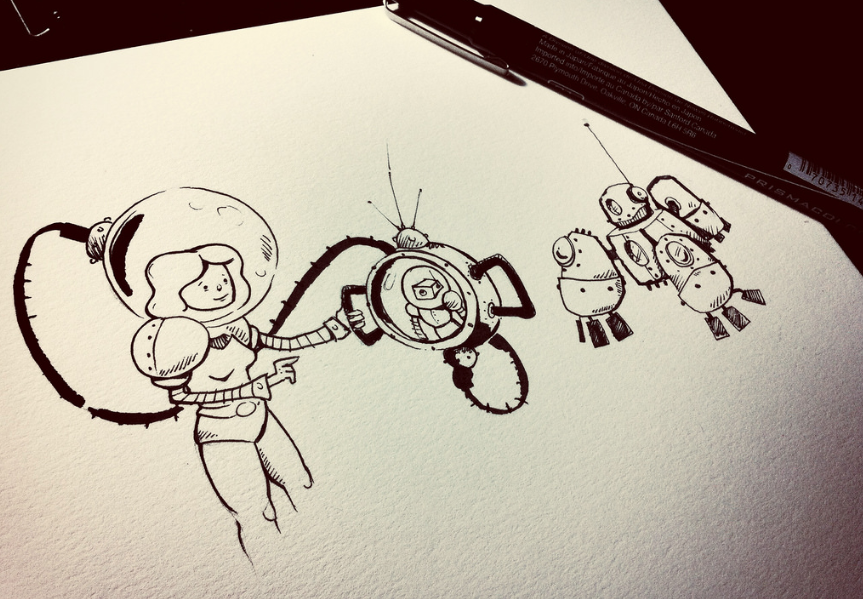
\includegraphics[width=\paperwidth,height=\paperheight]{figures/illustration.png}}
  \begin{frame}
  \end{frame}
}
%%%%%%%%%%%%%%%%%%%%%%%%%%%%%%%%%%%%%%%%%%%%%%%%%%%%%%%%%%%%%%%%%%%%%%%%%%%%%%%%
%%%%%%%%%%%%%%%%%%%%%%%%%%%%%%%%%%%%%%%%%%%%%%%%%%%%%%%%%%%%%%%%%%%%%%%%%%%%%%%%
\begin{frame}{Publications}
\begin{itemize}
\item
N. Dudebout and J. S. Shamma,
``Empirical Evidence Equilibria in Stochastic Games,''
in \emph{51st IEEE Conference on Decision and Control}, Dec. 2012, pp. 5780--5785
\item
N. Dudebout and J. S. Shamma,
``Exogenous Empirical-evidence Equilibria in Perfect-monitoring Repeated Games Yield Correlated Equilibria,''
in \emph{53rd IEEE Conference on Decision and Control}, Submitted
\item
N. Dudebout and J. S. Shamma,
``Empirical-evidence Equilibrium,''
in \emph{Games and Economic Behavior}, In Preparation
\end{itemize}
\end{frame}
%%%%%%%%%%%%%%%%%%%%%%%%%%%%%%%%%%%%%%%%%%%%%%%%%%%%%%%%%%%%%%%%%%%%%%%%%%%%%%%%
%%%%%%%%%%%%%%%%%%%%%%%%%%%%%%%%%%%%%%%%%%%%%%%%%%%%%%%%%%%%%%%%%%%%%%%%%%%%%%%%
\begin{frame}<2>{Endogenous Model}
\centertikz{endogenous_model}
\end{frame}
%%%%%%%%%%%%%%%%%%%%%%%%%%%%%%%%%%%%%%%%%%%%%%%%%%%%%%%%%%%%%%%%%%%%%%%%%%%%%%%%
%%%%%%%%%%%%%%%%%%%%%%%%%%%%%%%%%%%%%%%%%%%%%%%%%%%%%%%%%%%%%%%%%%%%%%%%%%%%%%%%
\begin{frame}{Brouwer's Fixed-point Theorem}
\centertikz{brouwer_theorem}
\end{frame}
%%%%%%%%%%%%%%%%%%%%%%%%%%%%%%%%%%%%%%%%%%%%%%%%%%%%%%%%%%%%%%%%%%%%%%%%%%%%%%%%
%%%%%%%%%%%%%%%%%%%%%%%%%%%%%%%%%%%%%%%%%%%%%%%%%%%%%%%%%%%%%%%%%%%%%%%%%%%%%%%%
\begin{frame}{Kakutani's Fixed-point Theorem}
\centertikz{kakutani_theorem}
\end{frame}
%%%%%%%%%%%%%%%%%%%%%%%%%%%%%%%%%%%%%%%%%%%%%%%%%%%%%%%%%%%%%%%%%%%%%%%%%%%%%%%%
%%%%%%%%%%%%%%%%%%%%%%%%%%%%%%%%%%%%%%%%%%%%%%%%%%%%%%%%%%%%%%%%%%%%%%%%%%%%%%%%
\begin{frame}{Consistency Formula}
\[
\mu \of {z} \elmt{s\nxt} = \sum\idx{w\nxt} \nu\of{w\nxt}\elmt{s\nxt} \frac{\sum\idx{w, x, a} \pi\strat{\sigma}\elmt{w,x,z} \mult \sigma \of{z} \elmt{a} \mult n \of{w,x,a} \elmt{w\nxt}}{\sum\idx{w, x} \pi\strat{\sigma}\elmt{w,x,z}}
\]
\end{frame}
%%%%%%%%%%%%%%%%%%%%%%%%%%%%%%%%%%%%%%%%%%%%%%%%%%%%%%%%%%%%%%%%%%%%%%%%%%%%%%%%
%%%%%%%%%%%%%%%%%%%%%%%%%%%%%%%%%%%%%%%%%%%%%%%%%%%%%%%%%%%%%%%%%%%%%%%%%%%%%%%%
\begin{frame}{Consistency}
\structure{Strong Consistency}
\\\medskip
\qquad\(\displaystyle \mu\of{z}\elmt{s\nxt} = \limfty{t} \probacond{S\Tp = s\nxt}{Z\Tt = z}\)
\\\bigskip\bigskip

\structure{Weak Consistency}\newinthesis
\\\medskip
\qquad\(\displaystyle \mu\of{z}\elmt{s\nxt} = \limfty{T} \frac{1}{T} \sum\idxfromto{t}{1}{T} \probacond{S\Tp = s\nxt}{Z\Tt = z}\)
\\\bigskip\bigskip

\structure{Eventual Consistency}\newinthesis
\\\medskip
\qquad\(\displaystyle \limfty{t} \probaof{Z\Tt = z} > 0 \implies \mu\of{z}\elmt{s\nxt} = \limfty{t} \probacond{S\Tp = s\nxt}{Z\Tt = z}\)
\end{frame}
%%%%%%%%%%%%%%%%%%%%%%%%%%%%%%%%%%%%%%%%%%%%%%%%%%%%%%%%%%%%%%%%%%%%%%%%%%%%%%%%
%%%%%%%%%%%%%%%%%%%%%%%%%%%%%%%%%%%%%%%%%%%%%%%%%%%%%%%%%%%%%%%%%%%%%%%%%%%%%%%%
\begin{frame}{Learning Result}
\begin{theorem}
Suppose the theoretical learning dynamic has a Lyapunov function.
For a large enough observation window, the empirical learning dynamic converges.
\end{theorem}

\begin{proof}
\begin{itemize}
\item ODE method for stochastic approximation
\item Lyapunov stability of perturbed systems
\end{itemize}
\end{proof}
\end{frame}
%%%%%%%%%%%%%%%%%%%%%%%%%%%%%%%%%%%%%%%%%%%%%%%%%%%%%%%%%%%%%%%%%%%%%%%%%%%%%%%%
}
